\begin{document}

\subsection{Biotronik Tour}

\outreachEntry{date}{Connect}{Dominik, Julia, Michael, Ori, Rachel, Sarah}{

\textbf{Summary:} Biotronik is a medical technology company that develops pacemakers and other electronics for various hospitals around the world. Biotronik was founded in 1963, in Berlin, Germany, and has spread around the world, with factories in over a hundred countries. During our tour of their factory in Lake Oswego, Oregon, we saw the different ways that they created, assembled, and tested each microchip that went into a pacemaker. As we moved through the factory, it was very clear that the amount of precision, and speed, was crucial to their success. There were rows of machines lined up, most feeding directly into one another. Most of the work there had been automated, with technicians checking up on each machine to make sure its doing its job correctly. Additionally, they had a mobile robot called SWIFT that was essentially a cart on wheels, that has on board cameras and navigation, that could automatically detect when a machine needs more parts, and then go get those parts, and deliver them without need for human intervention. After our group got back from the tour of the factory, we talked with our tour guide about what we do at robotics, and as it turns out he did robotics in college, and so we started talking about what each of us have done, and our different struggles in robotics, and how we've overcome them.

\textbf{Impact:} Biotronik showed us what real life industrial robots are capable of, and opened our eyes to all the things you can do with robotics if we choose to do this professionally. The precision they have achieved with their testing machines is truly remarkable, and really shows us how far we could take this if we wanted. Their autonomous robot, SWIFT, is very similar to what we do now, with vision, mechanisms for alignment, and navigation, which was all done on a tank drive, so it was interesting to see how much it could do, when we normally scoff at tank drives for their lack of flexibility.
\begin{center}
    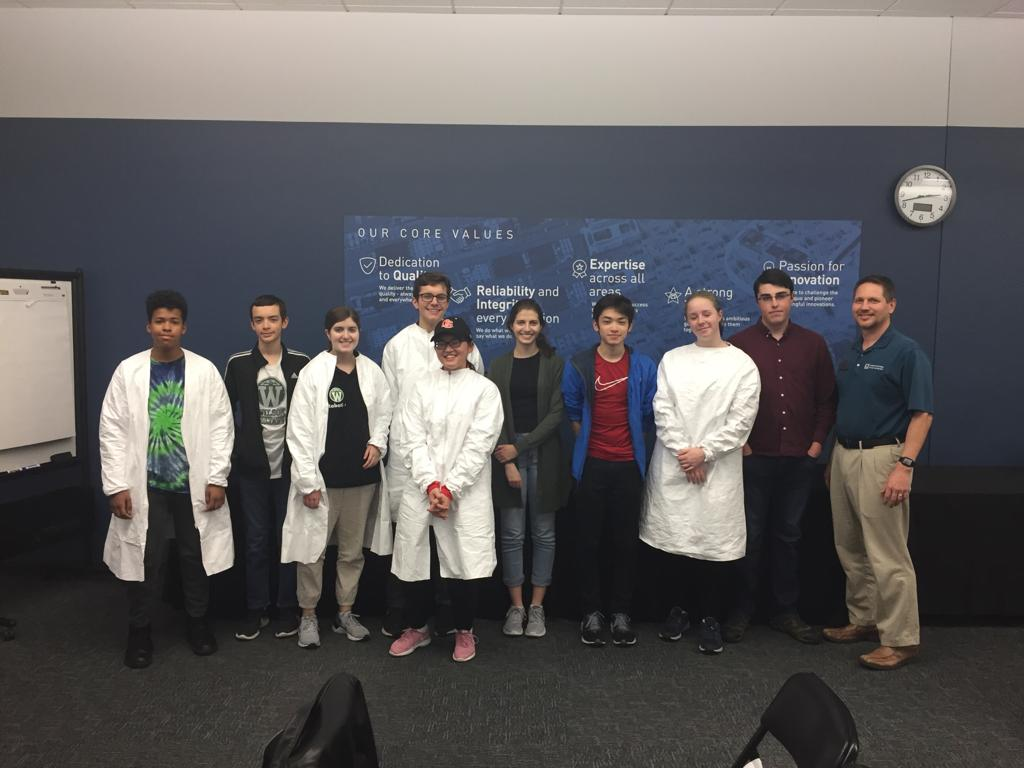
\includegraphics[width=.75\textwidth]{OutreachImages/Biotronik.jpeg}
\end{center}
}

\end{document}{}